A $\textrm{B}^+$Tree is a data structure that
can be used to map from keys to values. Figure \ref{b-tree} shows a tree that
maps from {\tt int}s to \texttt{String}s.

\begin{figure}[h]
\caption{A partially drawn $\textrm{B}^+$Tree of \texttt{String}s, keyed on \texttt{int}s}
\label{b-tree}
\center
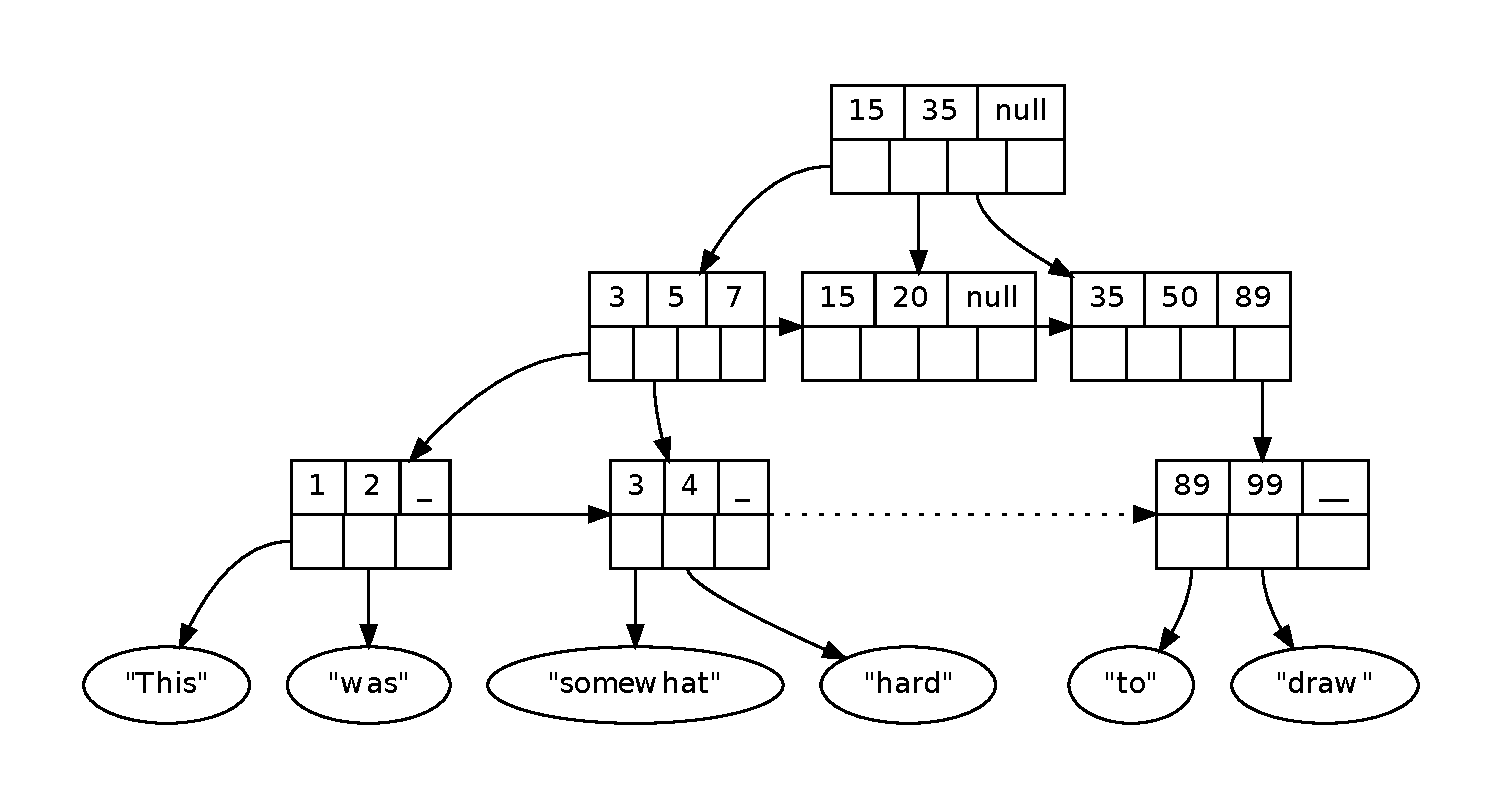
\includegraphics[width=5in]{other/b_plus_tree_dot.pdf}
\vspace{-1cm}
\end{figure}

    \begin{enumerate}
    \item What Java Collections Framework interface should a
    $\textrm{B}^+$Tree be able to implement?

        \begin{answer}
        \texttt{Java.util.Map$<$K,V$>$}
        \end{answer}
		\vspace{0.125in}

    \item We need to implement two different kinds of nodes for the tree. Why
    do we need to do this? What is different between the two types of nodes?

        \begin{answer}
        Some nodes (the leaves) point to data values. We also have internal
        nodes which point to other nodes (both internal nodes and leaves).
        \end{answer}
		\vspace{0.125in}

    \item We need classes to represent the nodes of the tree. Implement these
    classes so that they use generic types and all of their members are package
    private. Don't implement the constructors or any other methods.

\begin{answer}
\begin{lstlisting}
public interface BTreeNode<K,V> {}

public class InternalNode<K,V> implements BTreeNode<K,V>
{
    K[] keys;
    Node<K,V>[] children;
    InternalNode<K,V> next;
}

public class LeafNode<K,V> implements BTreeNode<K,V>
{
    K keys[];
    V values[];
    LeafNode<K,V> next;
}
\end{lstlisting}
\end{answer}

    \end{enumerate}